
\documentclass[12pt,a4paper]{article}
\usepackage[utf8]{inputenc}
\usepackage[T1]{fontenc}
\usepackage[polish]{babel}
\usepackage{amsmath, amssymb, amsfonts}
\usepackage{graphicx}
\usepackage{booktabs}
\usepackage{longtable}
\usepackage{geometry}
\usepackage{float}
\usepackage{hyperref}
\usepackage{caption}
\usepackage{subcaption}
\usepackage{array}
\geometry{margin=2.5cm}
\graphicspath{{figures/}}
\hypersetup{colorlinks=true, linkcolor=blue, urlcolor=blue, citecolor=blue}

\title{Optymalizacja portfelowa Markowitza z ograniczeniem kardynalności\\z wykorzystaniem metod metaheurystycznych}
\author{Jakub Mikołajczak 121732 \\
Mikołaj Białoskórski 121278 \\
Kinga Głódź 121349}
\date{\today}

\begin{document}
\maketitle


\begin{abstract}
Raport przedstawia rozwiązanie problemu optymalizacji portfelowej Markowitza z ograniczeniem kardynalności. Celem obliczeniowym jest minimalizacja wariancji portfela przy zadanej minimalnej oczekiwanej stopie zwrotu, braku krótkiej sprzedaży oraz ograniczeniu liczby aktywów w portfelu. Zastosowano trzy metaheurystyki: Simulated Annealing, Genetic Algorithm oraz Particle Swarm Optimization. Badanie obejmuje opis procesu generowania danych, formalizację problemu, konstrukcję eksperymentu, walidację wyników, analizę dywersyfikacji i interpretację wyników dla konkretnego zbioru danych syntetycznych.
\end{abstract}
\newpage
\tableofcontents
\newpage

\section{Wstęp}
Optymalizacja portfelowa jest jednym z klasycznych zagadnień finansów ilościowych. Model Markowitza pozwala formalnie opisać kompromis między oczekiwaną stopą zwrotu a ryzykiem portfela, mierzonym wariancją. W praktyce inwestorzy często nakładają dodatkowe ograniczenia, które nie występują w podstawowej postaci modelu. Jednym z nich jest ograniczenie kardynalności, czyli ograniczenie liczby aktywów o niezerowej wadze.

Dodanie ograniczenia kardynalności zmienia strukturę problemu. Klasyczny model bez tego warunku może być rozwiązany metodami programowania kwadratowego. Po dodaniu limitu liczby aktywów pojawia się komponent dyskretny: trzeba jednocześnie wskazać aktywa wchodzące do portfela i dobrać ich wagi. To uzasadnia wykorzystanie metaheurystyk.

\section{Cel projektu}
Celem projektu jest przygotowanie kompletnego procesu obliczeniowego, który wczytuje lub generuje dane, szacuje oczekiwane stopy zwrotu i macierz kowariancji, rozwiązuje problem minimalizacji wariancji portfela z ograniczeniem kardynalności, porównuje algorytmy SA, GA i PSO oraz zapisuje wyniki w postaci tabel, wykresów i raportu.

\section{Klasyczny model Markowitza}

Niech $n$ oznacza liczbę aktywów, $w \in \mathbb{R}^n$ wektor wag portfela, 
$\mu \in \mathbb{R}^n$ wektor oczekiwanych stóp zwrotu, a 
$\Sigma \in \mathbb{R}^{n \times n}$ macierz kowariancji stóp zwrotu. 
Oczekiwana stopa zwrotu portfela wynosi
\[
    \mu_p = \mu^\top w,
\]
natomiast wariancja portfela ma postać
\[
    \sigma_p^2 = w^\top \Sigma w.
\]

W klasycznej wersji zadanie minimalizacji wariancji przy zadanym poziomie oczekiwanej stopy zwrotu ma postać wypukłego problemu programowania kwadratowego, o ile macierz kowariancji $\Sigma$ jest dodatnio półokreślona, a ograniczenia mają charakter liniowy. Problem ten można zapisać jako
\[
    \min_w \; w^\top \Sigma w
\]
przy ograniczeniach
\[
    \mu^\top w \geq r_0, 
    \qquad 
    \sum_{i=1}^{n} w_i = 1,
    \qquad 
    w_i \geq 0 \quad \text{dla } i=1,\dots,n.
\]

Jest to problem programowania kwadratowego, ponieważ funkcja celu jest funkcją kwadratową wag portfela, natomiast ograniczenia są liniowe. Przy dodatniej półokreśloności macierzy $\Sigma$ funkcja celu jest wypukła, co oznacza, że każde minimum lokalne jest jednocześnie minimum globalnym. W konsekwencji klasyczny problem Markowitza można rozwiązywać za pomocą standardowych metod optymalizacji wypukłej, takich jak algorytmy programowania kwadratowego, metody punktu wewnętrznego lub metody aktywnego zbioru ograniczeń.

Z praktycznego punktu widzenia oznacza to, że dla klasycznej wersji modelu nie ma potrzeby stosowania metaheurystyk. Algorytmy takie jak symulowane wyżarzanie, algorytmy genetyczne czy PSO stają się uzasadnione dopiero wtedy, gdy do problemu zostaną dodane ograniczenia nieliniowe lub dyskretne, na przykład ograniczenie kardynalności portfela.

\section{Problem z ograniczeniem kardynalności}

W projekcie rozważany jest problem:
\[
    \min_w \; w^\top \Sigma w
\]
przy ograniczeniach:
\[
    \mu^\top w \geq r_0, 
    \qquad 
    \sum_{i=1}^{n} w_i = 1, 
    \qquad 
    w_i \geq 0 \quad \text{dla } i=1,\dots,n,
    \qquad 
    \|w\|_0 \leq A.
\]

Symbol $\|w\|_0$ oznacza liczbę niezerowych elementów wektora wag, a więc liczbę aktywów uwzględnionych w portfelu. Parametr $A$ określa maksymalną dopuszczalną liczbę takich aktywów. Ograniczenie
\[
    \|w\|_0 \leq A
\]
zwiększa praktyczną interpretowalność portfela, ponieważ prowadzi do konstrukcji portfeli składających się z ograniczonej liczby instrumentów. Jednocześnie powoduje ono utratę wypukłości zbioru dopuszczalnego, ponieważ warunek ten ma charakter dyskretny: wymaga wyboru podzbioru aktywów, które zostaną włączone do portfela.
Aby zobaczyć tę utratę wypukłości, wystarczy rozważyć przypadek $A=1$. Portfel inwestujący całość środków w aktywo pierwsze oraz portfel inwestujący całość środków w aktywo drugie spełniają ograniczenie kardynalności. Jednak ich kombinacja wypukła, na przykład portfel o wagach $(\frac{1}{2},\frac{1}{2})$, zawiera już dwa aktywa, a więc narusza warunek $\|w\|_0 \leq 1$. Oznacza to, że zbiór dopuszczalny nie jest wypukły.

\section{Proces generujący dane}
Dane w projekcie mają charakter syntetyczny. Ich celem nie jest odwzorowanie konkretnego rynku, lecz utworzenie kontrolowanego środowiska eksperymentalnego, w którym występują aktywa o różnych profilach ryzyka. Proces generujący dane można interpretować jako uproszczony wieloczynnikowy model stóp zwrotu:
\[
    r_{i,t} = \mu_i + \beta_i f_t + \varepsilon_{i,t},
\]
gdzie $r_{i,t}$ jest stopą zwrotu aktywa $i$ w chwili $t$, $\mu_i$ oznacza dryf aktywa, $f_t$ jest wspólnym czynnikiem rynkowym, $\beta_i$ mierzy wrażliwość aktywa na czynnik rynkowy, a $\varepsilon_{i,t}$ jest indywidualnym składnikiem losowym aktywa. Wspólny czynnik rynkowy $f_t$ reprezentuje ogólny ruch rynku w chwili $t$, wpływający jednocześnie na wiele aktywów. Można go interpretować jako uproszczony odpowiednik stopy zwrotu szerokiego indeksu rynkowego lub syntetyczny szok makroekonomiczny oddziałujący na cały zbiór instrumentów.

W typowym rozszerzeniu finansowym zmienność składnika losowego może być modelowana procesem GARCH(1,1):
\[
    \varepsilon_t = \sigma_t z_t, \qquad z_t \sim \mathcal{N}(0,1),
\]
\[
    \sigma_t^2 = \omega + \alpha \varepsilon_{t-1}^2 + \beta \sigma_{t-1}^2,
\]
przy założeniach $\omega>0$, $\alpha\ge 0$, $\beta\ge 0$ oraz zwykle $\alpha+\beta<1$. W takim modelu duże zaburzenia zwiększają przyszłą wariancję, co odzwierciedla skupianie zmienności obserwowane w szeregach finansowych. W przygotowanym zbiorze syntetycznym wykorzystano praktyczny odpowiednik tej idei: aktywa mają zróżnicowane poziomy zmienności i są dzielone na klasy konserwatywne, zrównoważone oraz agresywne według empirycznego odchylenia standardowego.

Podział na klasy aktywów ma znaczenie interpretacyjne. Aktywa konserwatywne mają najniższą zmienność, agresywne najwyższą, a zrównoważone znajdują się między nimi. Dzięki temu można sprawdzić, czy minimalizacja wariancji prowadzi przede wszystkim do wyboru aktywów defensywnych, czy też wymusza domieszkę aktywów bardziej zmiennych w celu spełnienia ograniczenia minimalnego zwrotu.

\section{Reprezentacja rozwiązania i obsługa ograniczeń}

Każdy kandydacki portfel reprezentowany jest jako wektor wag $w$. Niezależnie od zastosowanej metaheurystyki, po wygenerowaniu lub aktualizacji rozwiązania stosowana jest ta sama procedura naprawy, której celem jest przywrócenie wykonalności portfela względem ograniczeń modelu.

W pierwszym kroku wartości ujemne są zastępowane zerami. Następnie pozostawiane jest co najwyżej $A$ największych wag, a pozostałe wagi są zerowane. Na końcu cały wektor jest normalizowany tak, aby suma wag była równa jeden:
\[
    \sum_{i=1}^{n} w_i = 1.
\]
W ten sposób procedura zapewnia spełnienie ograniczenia braku krótkiej sprzedaży oraz ograniczenia kardynalności:
\[
    w_i \geq 0,
    \qquad
    \|w\|_0 \leq A.
\]

Jeżeli portfel nie spełnia warunku minimalnej oczekiwanej stopy zwrotu,
\[
    \mu^\top w \geq r_0,
\]
procedura naprawy może dodatkowo zwiększać udział aktywów o najwyższych oczekiwanych stopach zwrotu. Należy jednak zaznaczyć, że taka modyfikacja ma charakter heurystyczny: poprawia szansę uzyskania rozwiązania dopuszczalnego, ale nie gwarantuje znalezienia portfela optymalnego.

Znaczenie procedury naprawy można szczególnie łatwo zauważyć w przypadku algorytmu PSO. Cząstka w PSO przechowuje swoją pozycję jako wektor liczb rzeczywistych, co dobrze odpowiada ciągłemu charakterowi wag portfela. Jednocześnie taki wektor nie uwzględnia automatycznie dyskretnego ograniczenia kardynalności
\[
    \|w\|_0 \leq A.
\]
Dlatego po każdej aktualizacji pozycji cząstki, podobnie jak po wygenerowaniu nowego rozwiązania w SA lub GA, konieczne jest zastosowanie procedury naprawy, która zeruje nadmiarowe wagi i ponownie normalizuje portfel.

\section{Algorytmy i hiperparametry}
\subsection{Simulated Annealing}
W naszym przykładzie SA rozpoczyna od losowego portfela spełniającego ograniczenia. W każdej iteracji generowane jest lokalne zaburzenie wag, po czym portfel jest naprawiany. Jeżeli nowy portfel ma niższą wariancję, zostaje zaakceptowany. Jeżeli jest gorszy, może zostać przyjęty z prawdopodobieństwem zależnym od temperatury. W eksperymencie wykorzystano losowe próbkowanie kandydatów odpowiadające idei lokalnego przeszukiwania; w notebooku bazowym parametry SA obejmują $450$ iteracji, temperaturę początkową $T_0=1.0$, współczynnik chłodzenia $\alpha=0.995$ oraz skalę kroku $0.12$.

\subsection{Genetic Algorithm}
GA operuje na populacji portfeli. Osobnikiem jest wektor wag po procedurze naprawy. W projekcie zastosowano populację $45$ osobników, $80$ generacji, selekcję turniejową, krzyżowanie jednorodne, prawdopodobieństwo mutacji $0.12$ oraz elitaryzm na poziomie około $8\%$ populacji. Wygenerowane potomstwo jest zawsze naprawiane, aby spełniało ograniczenia portfelowe.

\subsection{Particle Swarm Optimization}
PSO wykorzystuje rój cząstek, z których każda przechowuje wektor wag i wektor prędkości. W notebooku bazowym zastosowano $45$ cząstek i $90$ iteracji. Parametr bezwładności wynosi $0.72$, parametr poznawczy $1.45$, a parametr społeczny $1.45$. Po aktualizacji pozycji cząstki wykonywana jest naprawa ograniczeń, ponieważ standardowy ruch PSO może wygenerować zbyt wiele niezerowych wag albo wagi niesumujące się do jednego.

\section{Projekt eksperymentu}
Eksperyment przeprowadzono dla $A \in \{2,3,5,10,15\}$. Dla każdej pary $(A,\text{algorytm})$ wykonano $30$ niezależnych przebiegów, co daje łącznie $450$ uruchomień algorytmów. Podstawowym kryterium jakości jest dzienna wariancja portfela przy spełnieniu ograniczeń. Dodatkowo analizowano czas działania, stabilność wyników i dywersyfikację.

Zwiększenie liczby przebiegów z $3$ do $30$ pozwala na bardziej wiarygodną ocenę stabilności wyników i ogranicza wpływ pojedynczych nietypowych uruchomień. Ma to szczególne znaczenie dla metaheurystyk, których rezultat może zależeć od inicjalizacji losowej oraz losowych decyzji podejmowanych w trakcie przeszukiwania przestrzeni rozwiązań.

\section{Metryki oceny}
Wariancja i zmienność nie są niezależnymi informacjami, ponieważ zmienność jest pierwiastkiem z wariancji:
\[
    \sigma_p = \sqrt{\sigma_p^2}.
\]
Wariancja jest bezpośrednią funkcją celu modelu Markowitza, natomiast zmienność jest raportowana pomocniczo, ponieważ jest bardziej intuicyjna interpretacyjnie i ma tę samą jednostkę co stopa zwrotu. Nie należy traktować tych metryk jako dwóch niezależnych kryteriów.

Indeks HHI, czyli Herfindahl--Hirschman Index, mierzy koncentrację wag portfela:
\[
    HHI = \sum_{i=1}^{n} w_i^2.
\]
Im wyższy HHI, tym bardziej skoncentrowany portfel. Efektywna liczba aktywów jest odwrotnością tego indeksu:
\[
    N_{eff} = \frac{1}{HHI}.
\]
Jeżeli portfel ma równe wagi w $k$ aktywach, wtedy $N_{eff}=k$.

\section{Wyniki eksperymentu}

\begin{table}[H]
\centering
\caption{Klasy aktywów w danych syntetycznych}
\begin{tabular}{p{0.28\textwidth}p{0.62\textwidth}}
\toprule
Klasa aktywów & Interpretacja w eksperymencie \\
\midrule
Konserwatywne & niższa zmienność idiosynkratyczna, zwykle preferowane przy minimalizacji wariancji \\
Zrównoważone & pośredni profil ryzyka i zwrotu \\
Agresywne & wyższa zmienność, potencjalnie wyższe oczekiwane stopy zwrotu \\
\bottomrule
\end{tabular}
\end{table}


Tabela zbiorcza wyników została rozbita na trzy części, aby oddzielić jakość rozwiązania, stabilność obliczeń i dywersyfikację portfeli. Tabele agregujące pokazują średnie, odchylenia standardowe, najlepsze i najgorsze wartości wyznaczone na podstawie $30$ przebiegów dla każdej pary $(A,\text{algorytm})$. Jeżeli w tabeli występuje najlepszy wynik, oznacza on najniższą dzienną wariancję uzyskaną w pojedynczym przebiegu danej konfiguracji.



\begin{table}[H]
\centering
\caption{Jakość rozwiązań: wariancja, zmienność i zwrot}
\resizebox{\textwidth}{!}{\begin{tabular}{lllllll}
\toprule
$A$ & Algorytm & Śr. wariancja dzienna & Najlepsza wariancja dzienna & Śr. zwrot roczny & Śr. zmienność roczna & Dopuszczalne \\
\midrule
2 & GA & 0{,}00004491 & 0{,}00004379 & 6{,}73\% & 10{,}64\% & 100\% \\
2 & PSO & 0{,}00004745 & 0{,}00004383 & 6{,}75\% & 10{,}89\% & 100\% \\
2 & SA & 0{,}00026378 & 0{,}00005136 & 9{,}91\% & 24{,}50\% & 100\% \\
3 & GA & 0{,}00003781 & 0{,}00003723 & 6{,}28\% & 9{,}76\% & 100\% \\
3 & PSO & 0{,}00003937 & 0{,}00003723 & 6{,}25\% & 9{,}96\% & 100\% \\
3 & SA & 0{,}00007377 & 0{,}00004401 & 6{,}46\% & 13{,}42\% & 100\% \\
5 & GA & 0{,}00003291 & 0{,}00003290 & 6{,}29\% & 9{,}11\% & 100\% \\
5 & PSO & 0{,}00003757 & 0{,}00003332 & 5{,}84\% & 9{,}72\% & 100\% \\
5 & SA & 0{,}00007056 & 0{,}00004493 & 6{,}80\% & 13{,}25\% & 100\% \\
10 & PSO & 0{,}00003293 & 0{,}00003120 & 5{,}81\% & 9{,}11\% & 100\% \\
10 & GA & 0{,}00003323 & 0{,}00003155 & 5{,}82\% & 9{,}15\% & 100\% \\
10 & SA & 0{,}00007316 & 0{,}00005209 & 6{,}70\% & 13{,}55\% & 100\% \\
15 & PSO & 0{,}00003263 & 0{,}00003120 & 5{,}81\% & 9{,}07\% & 100\% \\
15 & GA & 0{,}00003774 & 0{,}00003321 & 5{,}83\% & 9{,}75\% & 100\% \\
15 & SA & 0{,}00007847 & 0{,}00005468 & 6{,}58\% & 14{,}04\% & 100\% \\
\bottomrule
\end{tabular}
}
\end{table}

Porównanie wyników pokazuje, że algorytmy różnią się nie tylko jakością najlepszego 
znalezionego rozwiązania, lecz także powtarzalnością oraz kosztem obliczeniowym. 
Niższe odchylenie standardowe wariancji oznacza większą stabilność wyników między 
kolejnymi uruchomieniami, natomiast czas działania informuje o praktycznym koszcie 
zastosowania danej metody.

Z tego względu ocena algorytmów nie powinna ograniczać się do porównania minimalnej 
wariancji. Metoda, która uzyskuje bardzo dobry pojedynczy wynik, ale cechuje się dużą 
zmiennością rezultatów albo wysokim czasem obliczeń, może być mniej atrakcyjna 
praktycznie niż metoda dająca nieco gorsze, lecz bardziej stabilne wyniki.



\begin{table}[H]
\centering
\caption{Stabilność i czas działania algorytmów}
\resizebox{\textwidth}{!}{\begin{tabular}{lllllll}
\toprule
A & Alg. & Odch. war. & Mediana war. & Najg. war. & Czas [s] & Dopuszcz. \\
\midrule
2 & GA & 0.00e+00 & 0.00004438 & 0.00004438 & 0.3943 & 1.0000 \\
2 & PSO & 3.33e-05 & 0.00004649 & 0.00010373 & 0.4809 & 1.0000 \\
2 & SA & 2.31e-04 & 0.00027057 & 0.00057503 & 0.0735 & 1.0000 \\
3 & GA & 1.69e-06 & 0.00003723 & 0.00004015 & 0.3654 & 1.0000 \\
3 & PSO & 1.30e-06 & 0.00003793 & 0.00004018 & 0.2799 & 1.0000 \\
3 & SA & 3.69e-05 & 0.00012737 & 0.00014178 & 0.0382 & 1.0000 \\
5 & GA & 5.36e-09 & 0.00003291 & 0.00003291 & 0.3468 & 1.0000 \\
5 & PSO & 3.40e-06 & 0.00003383 & 0.00003952 & 0.7389 & 1.0000 \\
5 & SA & 1.66e-05 & 0.00005431 & 0.00007812 & 0.0303 & 1.0000 \\
10 & PSO & 1.10e-06 & 0.00003293 & 0.00003365 & 0.4704 & 1.0000 \\
10 & GA & 1.37e-06 & 0.00003265 & 0.00003495 & 0.5559 & 1.0000 \\
10 & SA & 1.26e-05 & 0.00007646 & 0.00008780 & 0.0658 & 1.0000 \\
15 & PSO & 2.62e-06 & 0.00003190 & 0.00003621 & 0.6772 & 1.0000 \\
15 & GA & 4.18e-07 & 0.00003760 & 0.00003765 & 0.3796 & 1.0000 \\
15 & SA & 5.23e-06 & 0.00008506 & 0.00009139 & 0.0331 & 1.0000 \\
\bottomrule
\end{tabular}
}
\end{table}


\begin{table}[H]
\centering
\caption{Dywersyfikacja i udział klas aktywów}
\resizebox{\textwidth}{!}{\begin{tabular}{llllllll}
\toprule
$A$ & Algorytm & Śr. efektywna liczba aktywów & Śr. HHI & Śr. maks. waga & Konserwatywne & Zrównoważone & Agresywne \\
\midrule
2 & GA & 1{,}99 & 0{,}5023 & 53{,}16\% & 100{,}0\% & 0{,}0\% & 0{,}0\% \\
2 & PSO & 1{,}97 & 0{,}5070 & 54{,}24\% & 98{,}6\% & 1{,}4\% & 0{,}0\% \\
2 & SA & 1{,}79 & 0{,}5700 & 64{,}80\% & 39{,}5\% & 38{,}7\% & 21{,}8\% \\
3 & GA & 2{,}96 & 0{,}3375 & 37{,}62\% & 100{,}0\% & 0{,}0\% & 0{,}0\% \\
3 & PSO & 2{,}83 & 0{,}3570 & 40{,}70\% & 99{,}8\% & 0{,}0\% & 0{,}2\% \\
3 & SA & 2{,}24 & 0{,}4651 & 57{,}33\% & 86{,}2\% & 9{,}6\% & 4{,}2\% \\
5 & GA & 4{,}86 & 0{,}2060 & 25{,}61\% & 100{,}0\% & 0{,}0\% & 0{,}0\% \\
5 & PSO & 3{,}86 & 0{,}2676 & 34{,}89\% & 98{,}9\% & 0{,}6\% & 0{,}5\% \\
5 & SA & 4{,}23 & 0{,}2390 & 32{,}10\% & 73{,}0\% & 20{,}9\% & 6{,}1\% \\
10 & PSO & 5{,}45 & 0{,}1876 & 23{,}84\% & 99{,}8\% & 0{,}1\% & 0{,}1\% \\
10 & GA & 6{,}99 & 0{,}1447 & 19{,}56\% & 97{,}7\% & 0{,}7\% & 1{,}6\% \\
10 & SA & 8{,}10 & 0{,}1246 & 20{,}19\% & 62{,}5\% & 27{,}9\% & 9{,}6\% \\
15 & PSO & 5{,}62 & 0{,}1817 & 22{,}85\% & 99{,}8\% & 0{,}1\% & 0{,}1\% \\
15 & GA & 9{,}18 & 0{,}1106 & 16{,}66\% & 90{,}3\% & 6{,}7\% & 3{,}0\% \\
15 & SA & 11{,}23 & 0{,}0902 & 15{,}48\% & 55{,}6\% & 31{,}2\% & 13{,}2\% \\
\bottomrule
\end{tabular}
}
\end{table}

\newpage

Tabela dotycząca dywersyfikacji pokazuje, w jakim stopniu uzyskane portfele są 
skoncentrowane w niewielkiej liczbie aktywów. Wartości w tej tabeli są średnimi po 
$30$ przebiegach dla danej pary $(A,\text{algorytm})$, dlatego nie należy interpretować 
ich jako parametrów jednego konkretnego portfela. Najlepsze pojedyncze przebiegi są 
wyznaczane w notebooku osobno, za pomocą wyboru najniższej dziennej wariancji dla 
każdego algorytmu. Takie rozróżnienie jest istotne, ponieważ konfiguracja o najlepszym 
pojedynczym wyniku nie musi być jednocześnie konfiguracją najbardziej stabilną, 
najszybszą albo najbardziej zdywersyfikowaną.

Dominacja aktywów o niższej zmienności jest zgodna z celem optymalizacji. Ponieważ 
w wariancie podstawowym minimalizowana jest wariancja portfela, algorytm naturalnie 
preferuje instrumenty o niższym poziomie ryzyka, o ile pozwalają one jednocześnie 
spełnić warunek minimalnej oczekiwanej stopy zwrotu.

\begin{figure}[H]
\centering
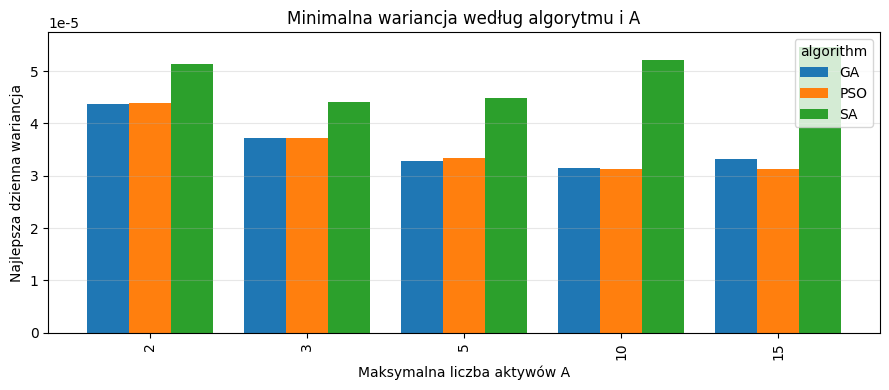
\includegraphics[width=0.9\textwidth]{min_variance_algorithms.png}
\caption{Najlepsza dzienna wariancja według algorytmu i ograniczenia kardynalności}
\end{figure}

\begin{figure}[H]
\centering
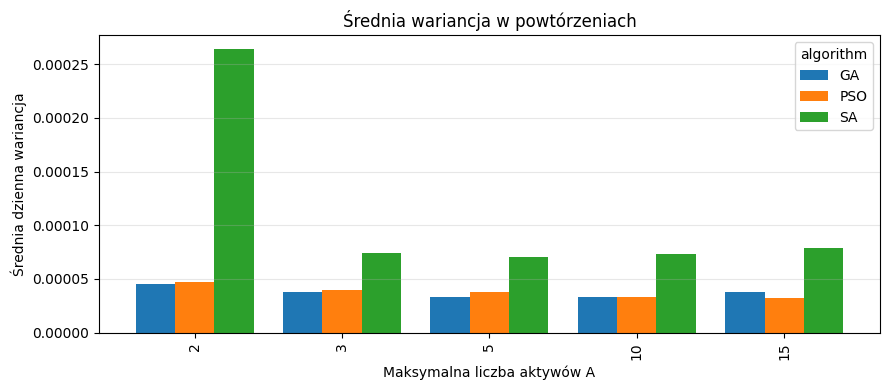
\includegraphics[width=0.9\textwidth]{sr_var_pow.png}
\caption{Średnia dzienna wariancja po 30 przebiegach}
\end{figure}

\begin{figure}[H]
\centering
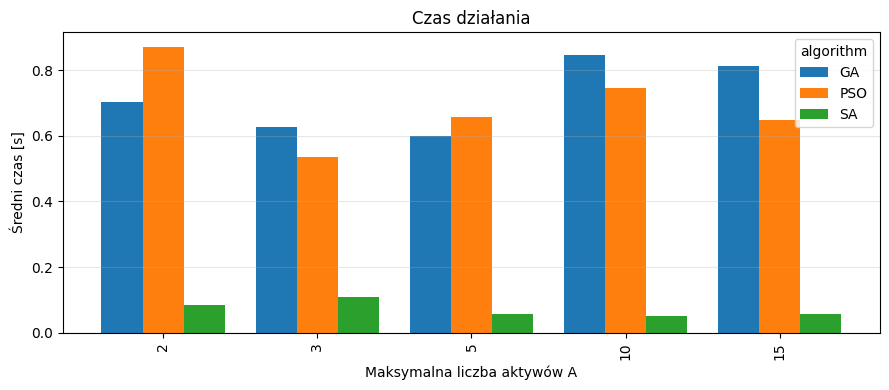
\includegraphics[width=0.9\textwidth]{runtime_algorithms.png}
\caption{Porównanie średniego czasu działania algorytmów po 30 przebiegach}
\end{figure}

\begin{figure}[H]
\centering
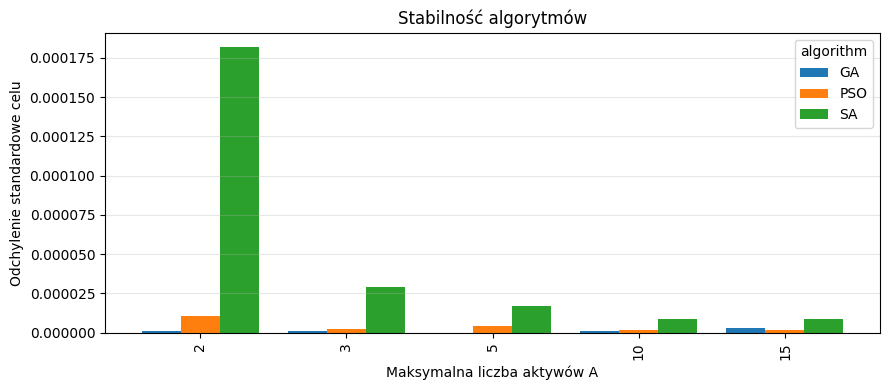
\includegraphics[width=0.9\textwidth]{stability_algorithms.png}
\caption{Stabilność algorytmów mierzona odchyleniem standardowym wartości funkcji celu}
\end{figure}

\section{Dywersyfikacja i skład portfela}
Dywersyfikacja jest istotna, ponieważ portfel o niskiej wariancji może być jednocześnie silnie skoncentrowany w niewielkiej liczbie aktywów. W przeprowadzonym eksperymencie portfele dla $A=2$ mają efektywną liczbę aktywów bliską dwóm, co jest naturalną konsekwencją bardzo silnego ograniczenia kardynalności. Dla wyższych wartości $A$ efektywna liczba aktywów zazwyczaj rośnie, lecz nie zawsze osiąga wartość równą samemu limitowi $A$. Wynika to z faktu, że minimalizacja wariancji może preferować większą koncentrację wag w kilku relatywnie stabilnych aktywach zamiast równomiernego rozłożenia kapitału na wszystkie dopuszczalne instrumenty.

Na podstawie uzyskanych wyników można zauważyć, że algorytm SA osiągał przeciętnie wyższą wariancję niż PSO oraz GA, niezależnie od przyjętej wartości $A$. Oznacza to, że w analizowanej konfiguracji SA radził sobie słabiej z minimalizacją wariancji portfela. Wniosek ten należy jednak odnosić do zastosowanych danych, parametrów algorytmów oraz liczby przeprowadzonych uruchomień.

\begin{figure}[H]
\centering
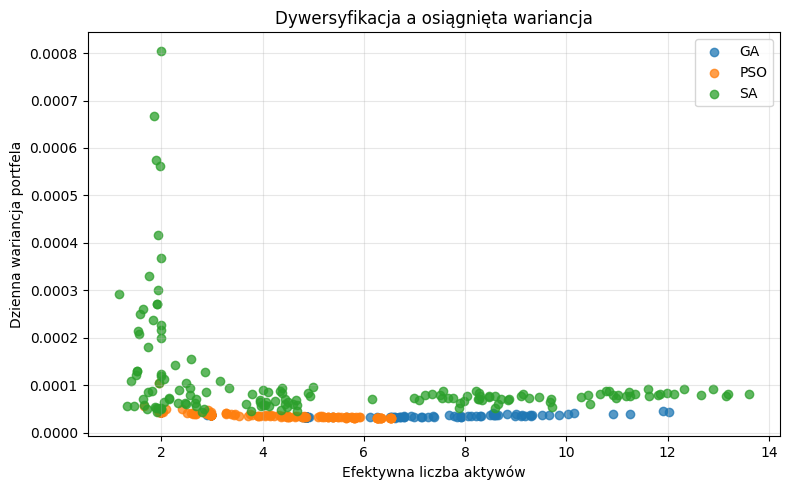
\includegraphics[width=0.85\textwidth]{diversification_vs_variance.png}
\caption{Relacja dywersyfikacji i dziennej wariancji dla pojedynczych przebiegów}
\end{figure}

\begin{figure}[H]
\centering
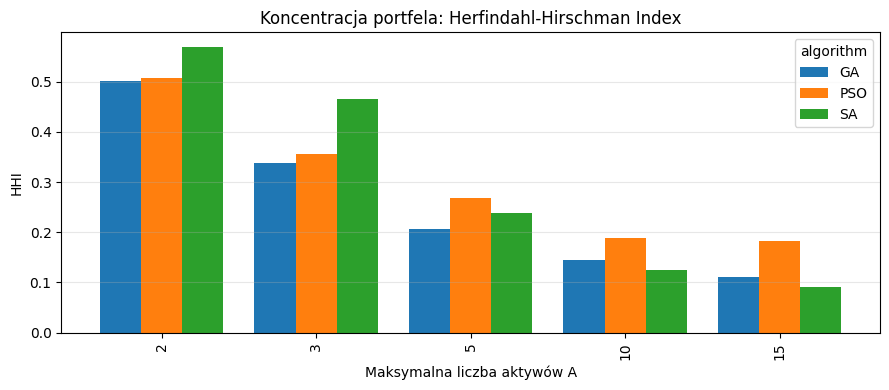
\includegraphics[width=0.85\textwidth]{hhi.png}
\caption{Średnia koncentracja portfela: Herfindahl--Hirschman Index}
\end{figure}

\begin{figure}[H]
\centering
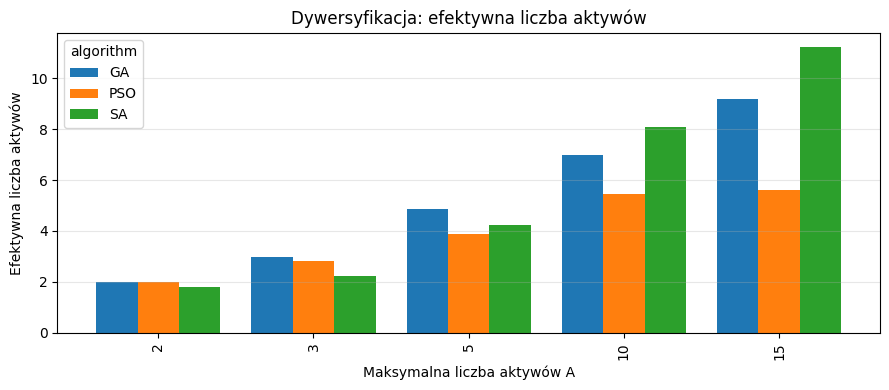
\includegraphics[width=0.85\textwidth]{eff.png}
\caption{Średnia efektywna liczba aktywów}
\end{figure}

\begin{figure}[H]
\centering
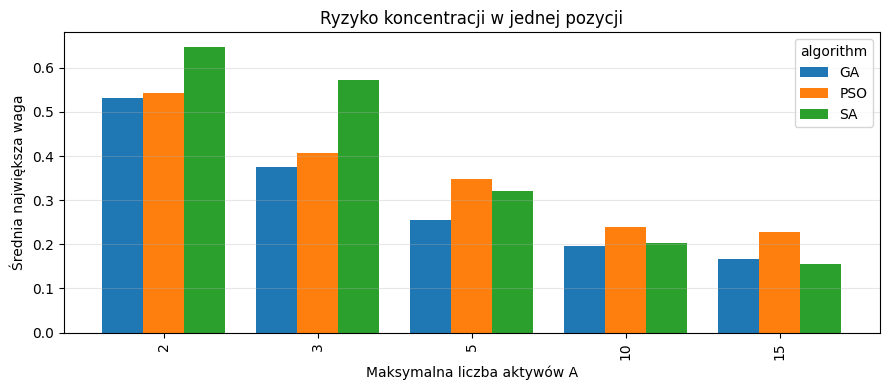
\includegraphics[width=0.85\textwidth]{max_weight.png}
\caption{Średnia największa pojedyncza waga w portfelu}
\end{figure}

\begin{figure}[H]
\centering
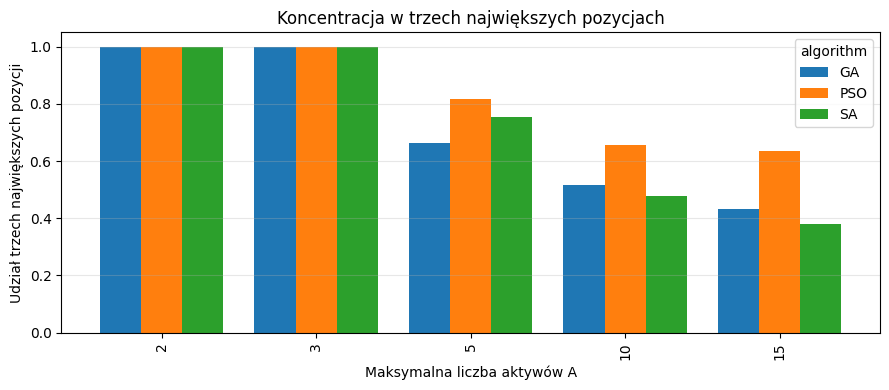
\includegraphics[width=0.85\textwidth]{top3_weight.png}
\caption{Średni udział trzech największych pozycji w portfelu}
\end{figure}

\begin{figure}[H]
\centering
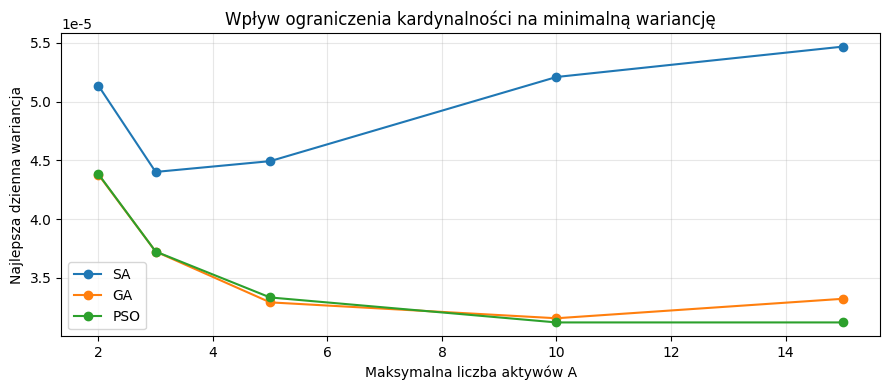
\includegraphics[width=0.85\textwidth]{ogr_kar_var.png}
\caption{Wpływ ograniczenia kardynalności na najlepszą dzienną wariancję}
\end{figure}

\begin{figure}[H]
\centering

\includegraphics[width=0.85\textwidth]{asset_classes_A2.png}
\caption{Średni udział klas aktywów w portfelach dla $A=2$}
\end{figure}

\begin{figure}[H]
\centering

\includegraphics[width=0.85\textwidth]{asset_classes_A3.png}
\caption{Średni udział klas aktywów w portfelach dla $A=3$}
\end{figure}

\begin{figure}[H]
\centering

\includegraphics[width=0.85\textwidth]{asset_classes_A5.png}
\caption{Średni udział klas aktywów w portfelach dla $A=5$}
\end{figure}

\begin{figure}[H]
\centering

\includegraphics[width=0.85\textwidth]{asset_classes_A10.png}
\caption{Średni udział klas aktywów w portfelach dla $A=10$}
\end{figure}

\begin{figure}[H]
\centering

\includegraphics[width=0.85\textwidth]{asset_classes_A15.png}
\caption{Średni udział klas aktywów w portfelach dla $A=15$}
\end{figure}

\begin{figure}[H]
\centering

\includegraphics[width=0.85\textwidth]{best_portfolio_weights.png}
\caption{Wagi najlepszego pojedynczego portfela według minimalnej dziennej wariancji}
\end{figure}

\begin{figure}[H]
\centering

\includegraphics[width=0.85\textwidth]{best_run_convergence.png}
\caption{Zbieżność algorytmu dla najlepszego ustawienia i uruchomienia wskazanego w notebooku}
\end{figure}

\section{Walidacja wyników}
Dla każdego z $450$ przebiegów sprawdzono sumę wag, nieujemność, ograniczenie kardynalności, minimalny oczekiwany zwrot oraz poprawność macierzy kowariancji. W aktualnym uruchomieniu wszystkie sprawdzone rozwiązania spełniły ograniczenia, czyli odsetek dopuszczalnych przebiegów wyniósł $100\%$. Walidacja jest konieczna, ponieważ sama niska wartość funkcji celu nie wystarcza, jeżeli portfel narusza ograniczenia formalne.

\section{Uwagi krytyczne i ograniczenia badania}
Wyniki należy interpretować ostrożnie. Dane mają charakter syntetyczny, więc nie są rekomendacją inwestycyjną. Metaheurystyki zależą od ziarna losowego, liczby kandydatów i hiperparametrów. Procedura naprawy ograniczeń wpływa na przeszukiwaną przestrzeń rozwiązań. Minimalizacja wariancji nie opisuje wszystkich aspektów ryzyka, szczególnie przy rozkładach skośnych lub z grubymi ogonami.

\section{Wnioski końcowe}
Z perspektywy projektu najważniejszy wniosek jest taki, że dodanie ograniczenia 
kardynalności istotnie zmienia charakter klasycznego problemu Markowitza. Problem 
przestaje być standardowym zadaniem wypukłego programowania kwadratowego, ponieważ 
oprócz doboru wag portfela pojawia się dyskretna decyzja o wyborze aktywów. W efekcie 
zadanie nabiera charakteru kombinatorycznego, co uzasadnia zastosowanie metaheurystyk.

W notebooku najlepsze pojedyncze wyniki są wyznaczane osobno dla każdego algorytmu 
przez posortowanie wszystkich przebiegów według dziennej wariancji. W tym ujęciu PSO 
osiąga najlepszy pojedynczy wynik przy $A=15$, GA przy $A=10$, a SA przy $A=3$. Nie oznacza 
to jednak, że jeden algorytm jest najlepszy we wszystkich kryteriach. Kod notebooka 
oddzielnie wskazuje konfigurację najszybszą średnio, najstabilniejszą według odchylenia 
wartości celu oraz najbardziej zdywersyfikowaną według średniej efektywnej liczby aktywów. 
Pełna ocena jakości algorytmów powinna więc uwzględniać nie tylko najlepszą uzyskaną 
wartość funkcji celu, lecz także stabilność rezultatów, czas działania, spełnienie 
ograniczeń oraz poziom dywersyfikacji portfela.

Wyniki wskazują również, że ograniczenie kardynalności pełni podwójną rolę. Z jednej 
strony zwiększa praktyczną interpretowalność portfela, ponieważ ogranicza liczbę 
utrzymywanych pozycji. Z drugiej strony utrudnia problem optymalizacyjny, ponieważ 
wymaga jednoczesnego rozwiązania problemu wyboru aktywów oraz alokacji wag.
\newpage
\begin{thebibliography}{9}
\bibitem{markowitz1952} H. Markowitz, Portfolio Selection, \textit{The Journal of Finance}, 7(1), 77--91, 1952.
\bibitem{kirkpatrick1983} S. Kirkpatrick, C. D. Gelatt, M. P. Vecchi, Optimization by Simulated Annealing, \textit{Science}, 220(4598), 671--680, 1983.
\bibitem{goldberg1989} D. E. Goldberg, \textit{Genetic Algorithms in Search, Optimization and Machine Learning}, Addison-Wesley, 1989.
\bibitem{kennedy1995} J. Kennedy, R. Eberhart, Particle Swarm Optimization, \textit{Proceedings of ICNN'95}, 1995.
\end{thebibliography}
\end{document}
